\section{Inverse Nonlinear Fourier Transform}
\begin{frame}{Roadmap}
    \begin{figure}
        \centering
        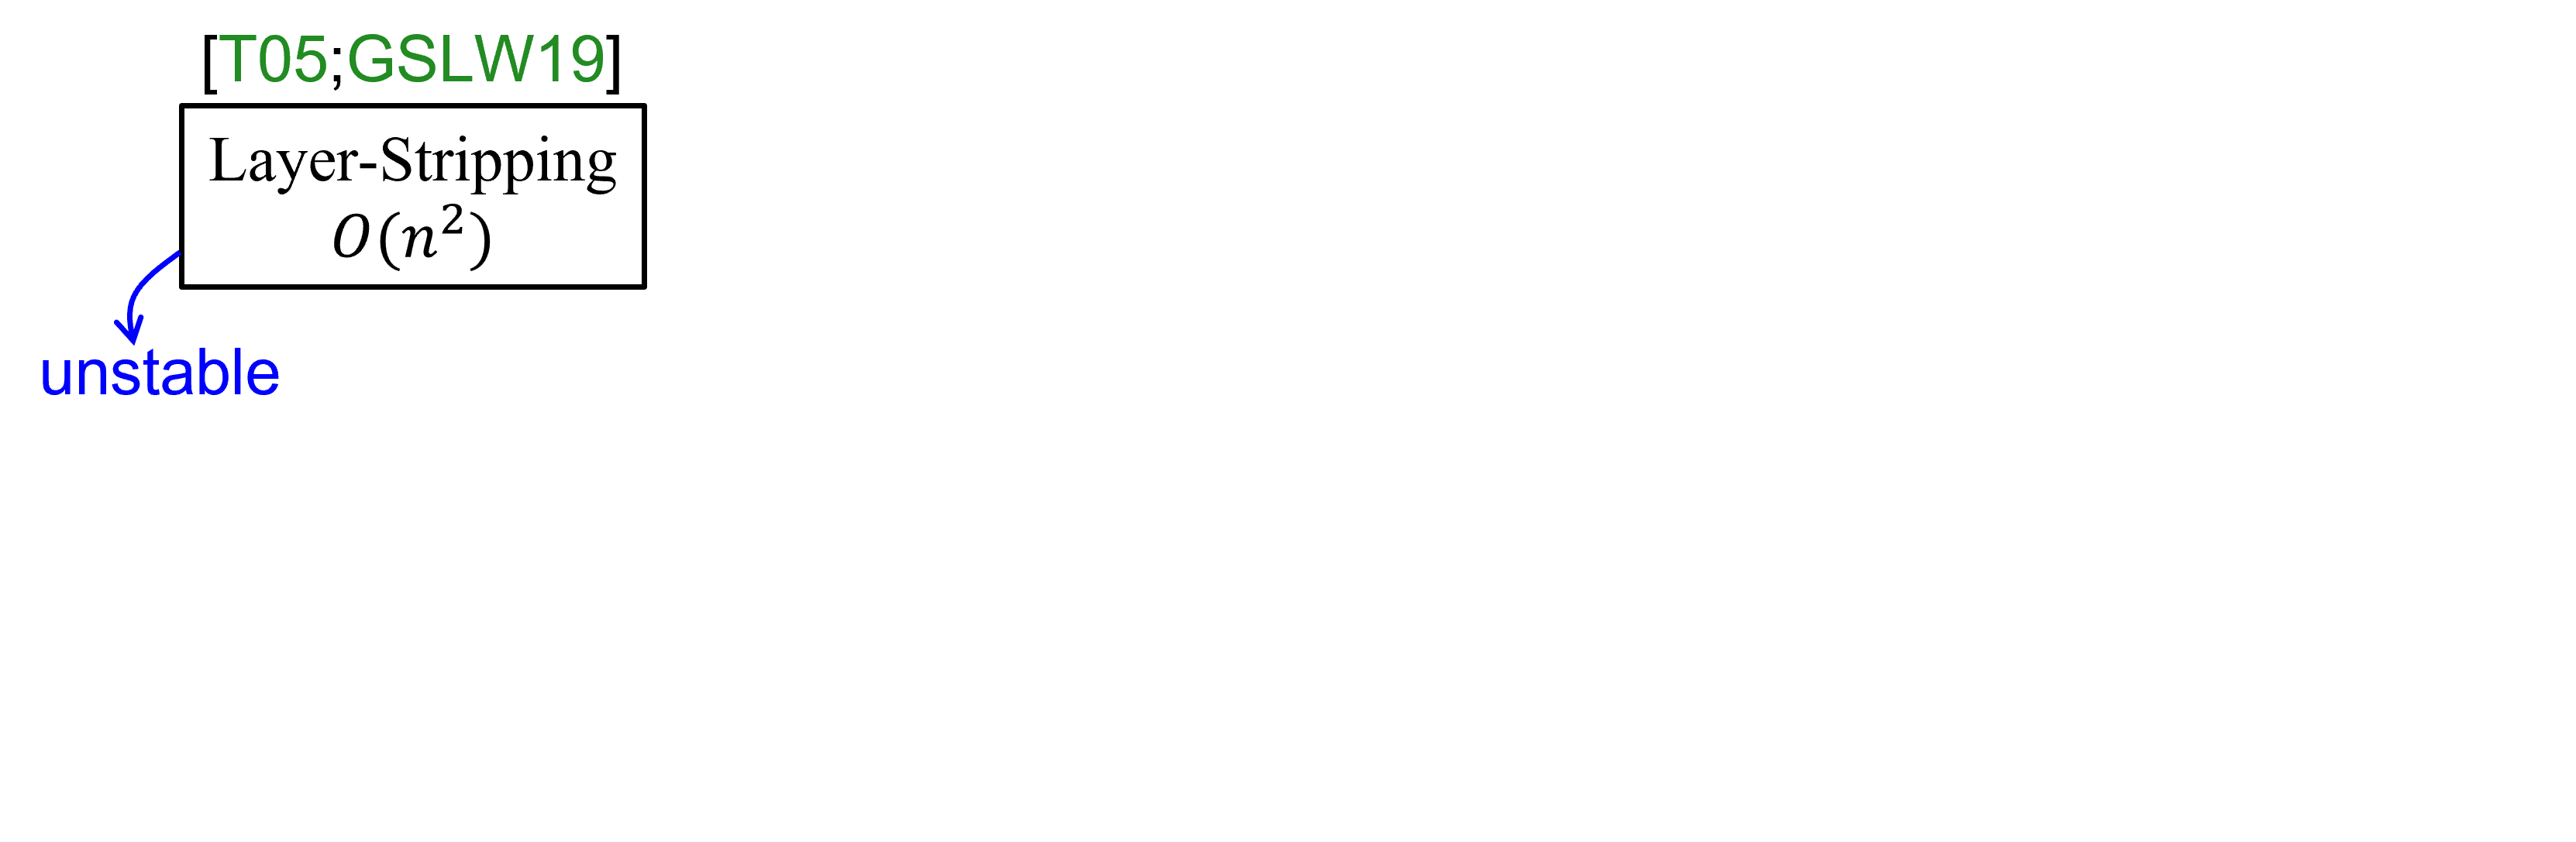
\includegraphics[width=1\linewidth]{figures/roadmap1.png}
    \end{figure}
\end{frame}
\addtocounter{framenumber}{-1}
\begin{frame}{Roadmap}
    \begin{figure}
        \centering
        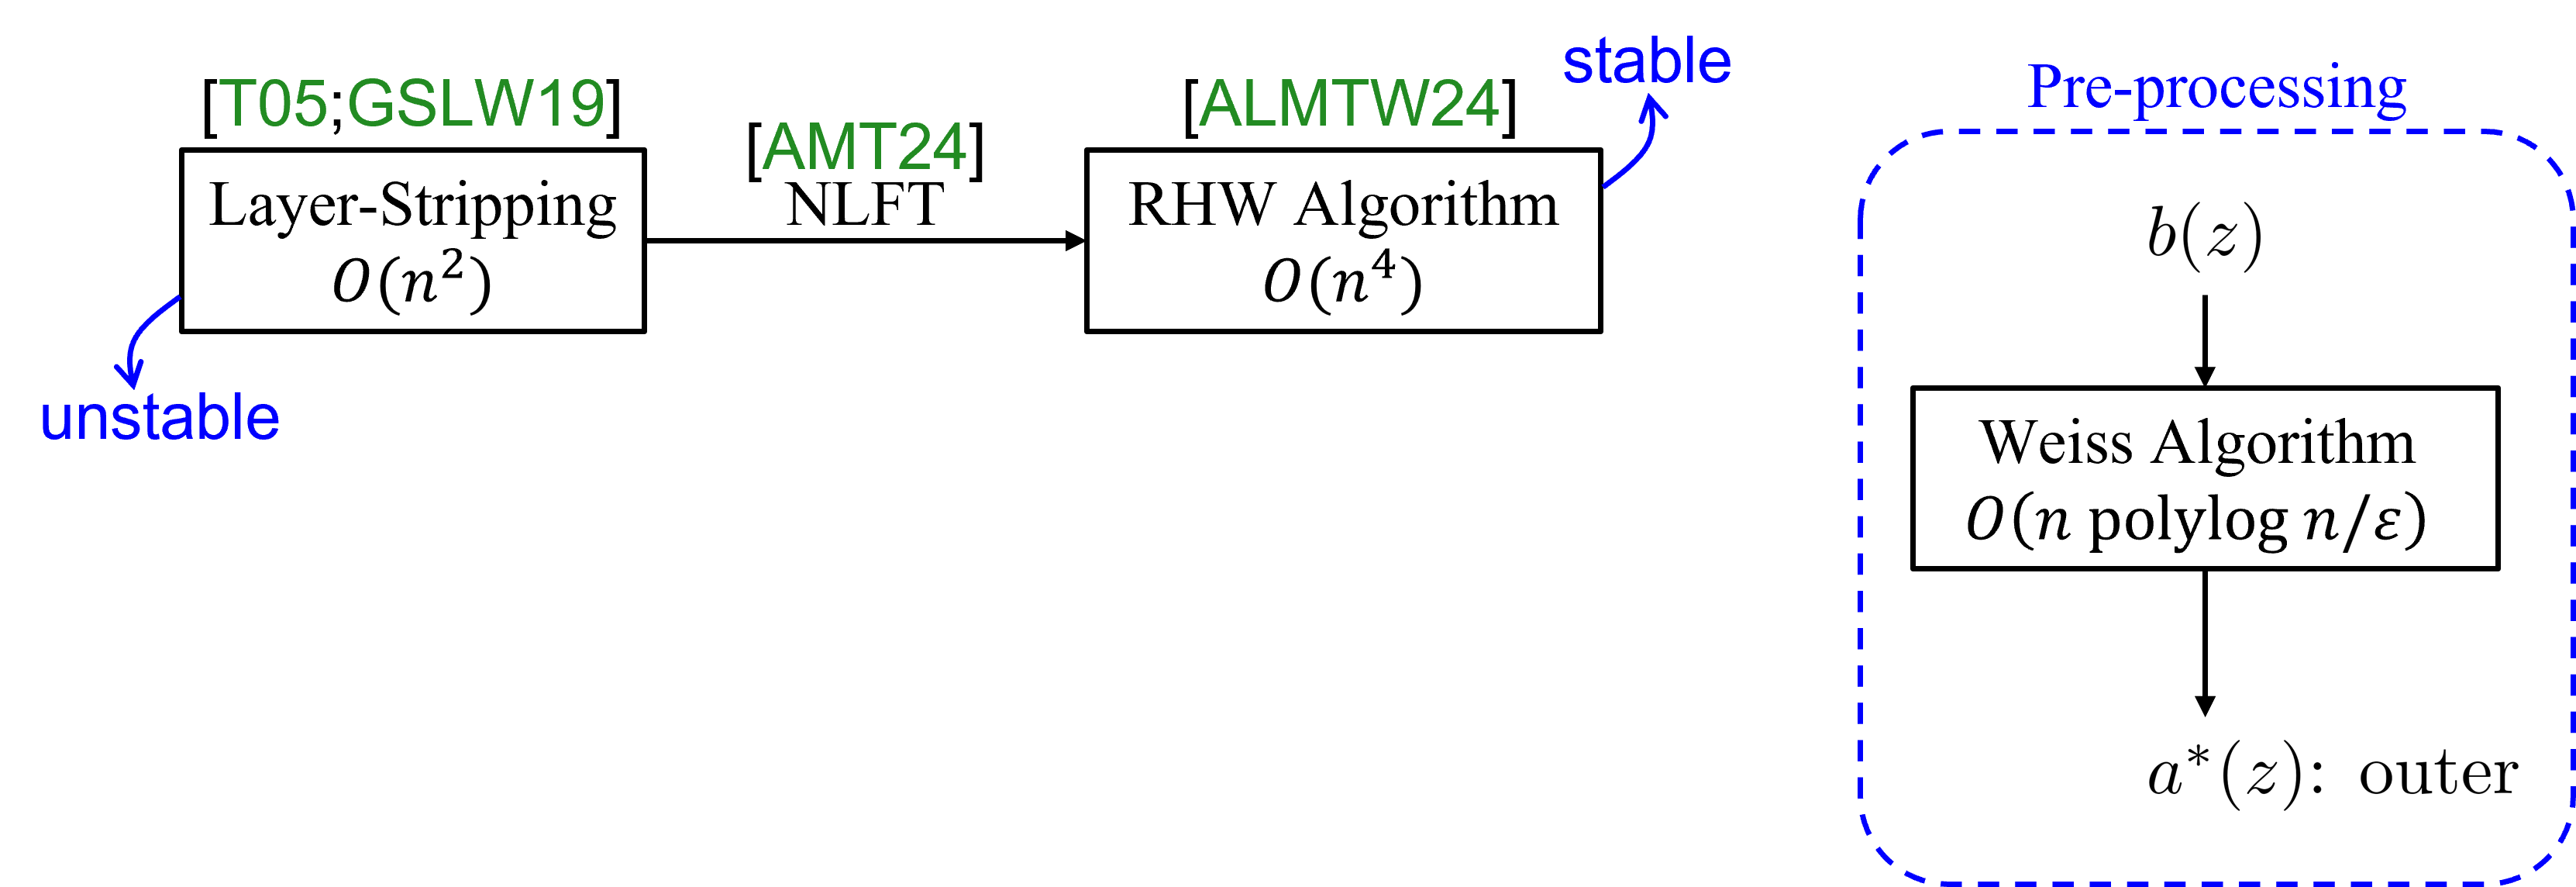
\includegraphics[width=1\linewidth]{figures/roadmap2.png}
    \end{figure}
\end{frame}
\addtocounter{framenumber}{-1}
\begin{frame}{Roadmap}
    \begin{figure}
        \centering
        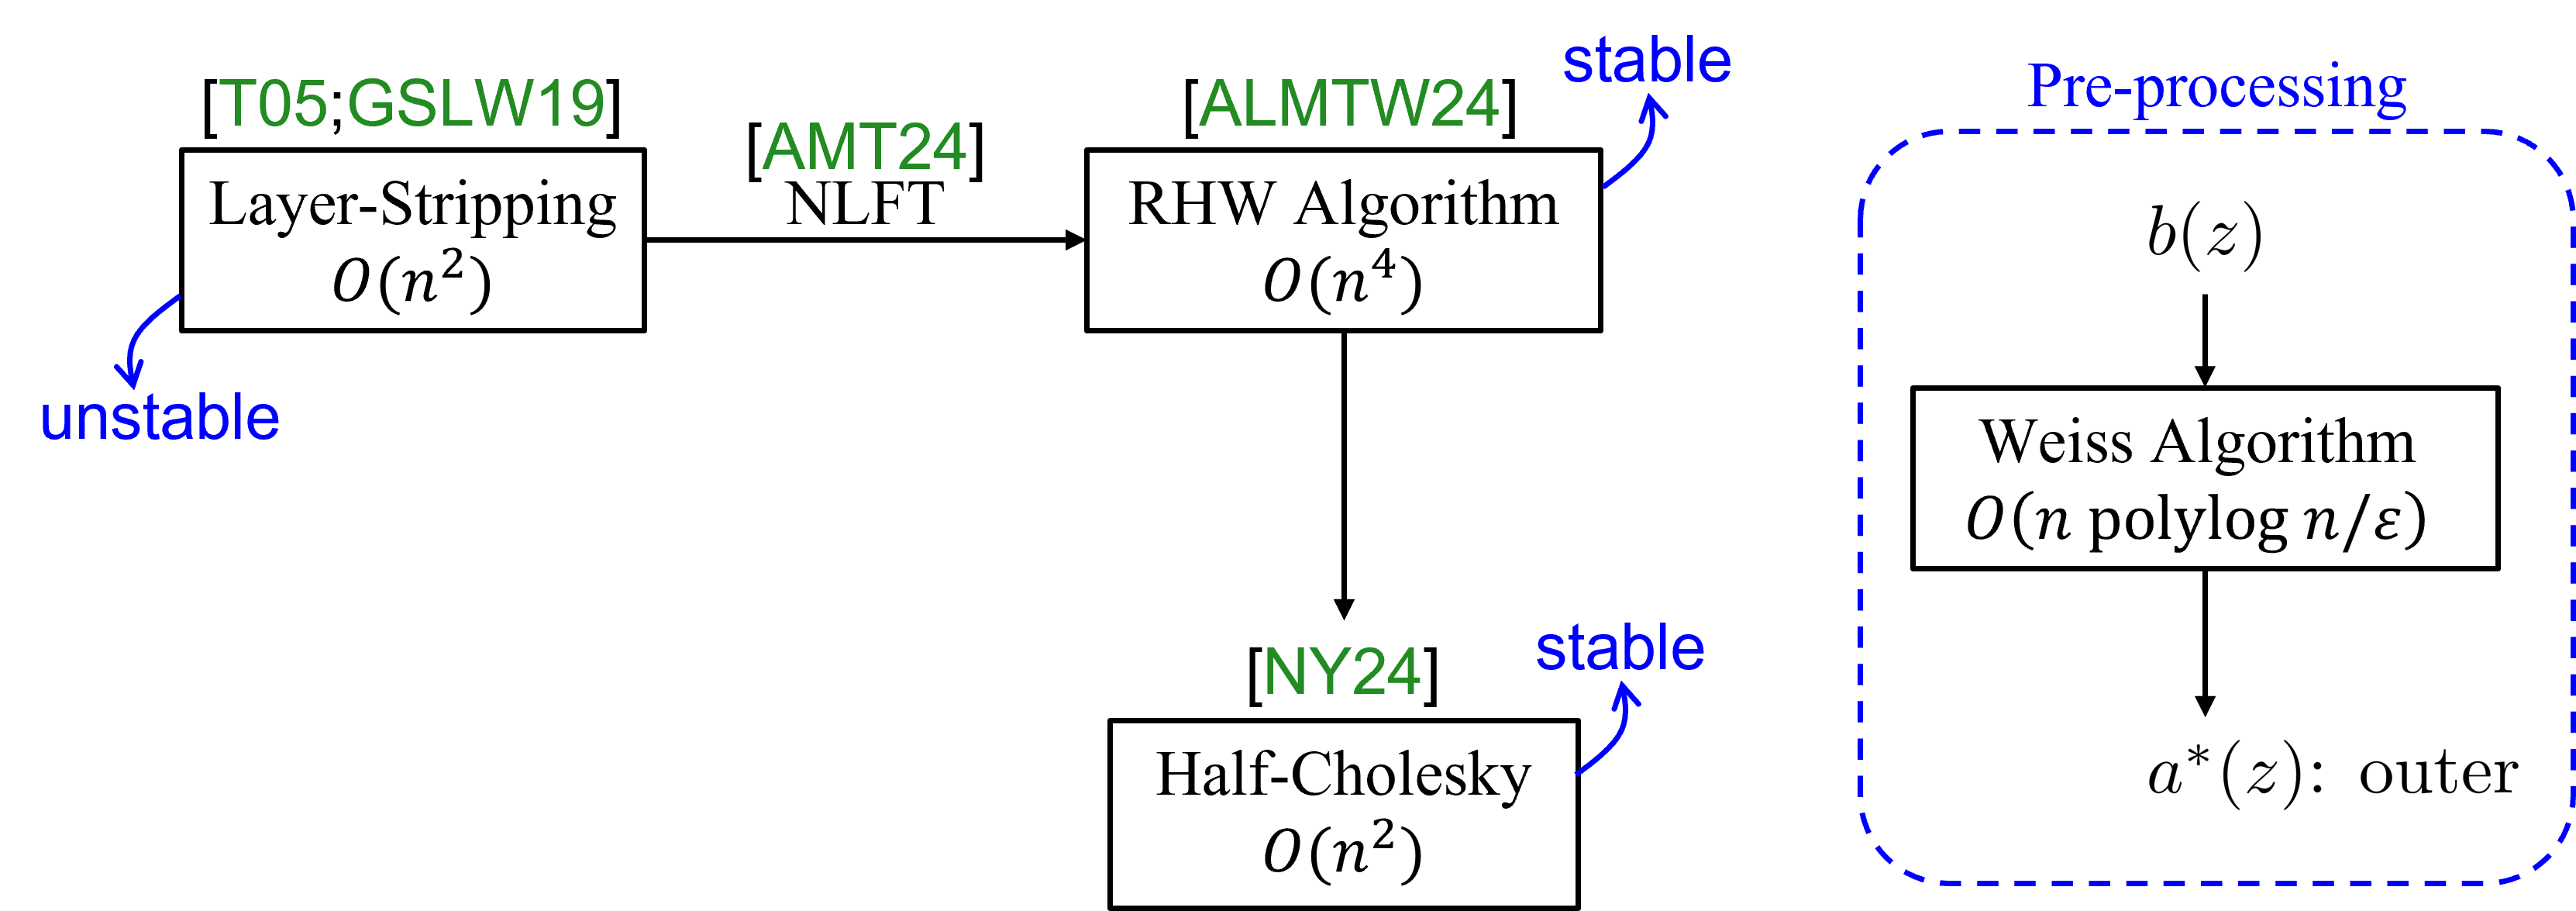
\includegraphics[width=1\linewidth]{figures/roadmap3.png}
    \end{figure}
\end{frame}
\addtocounter{framenumber}{-1}
\begin{frame}{Roadmap}
    \begin{figure}
        \centering
        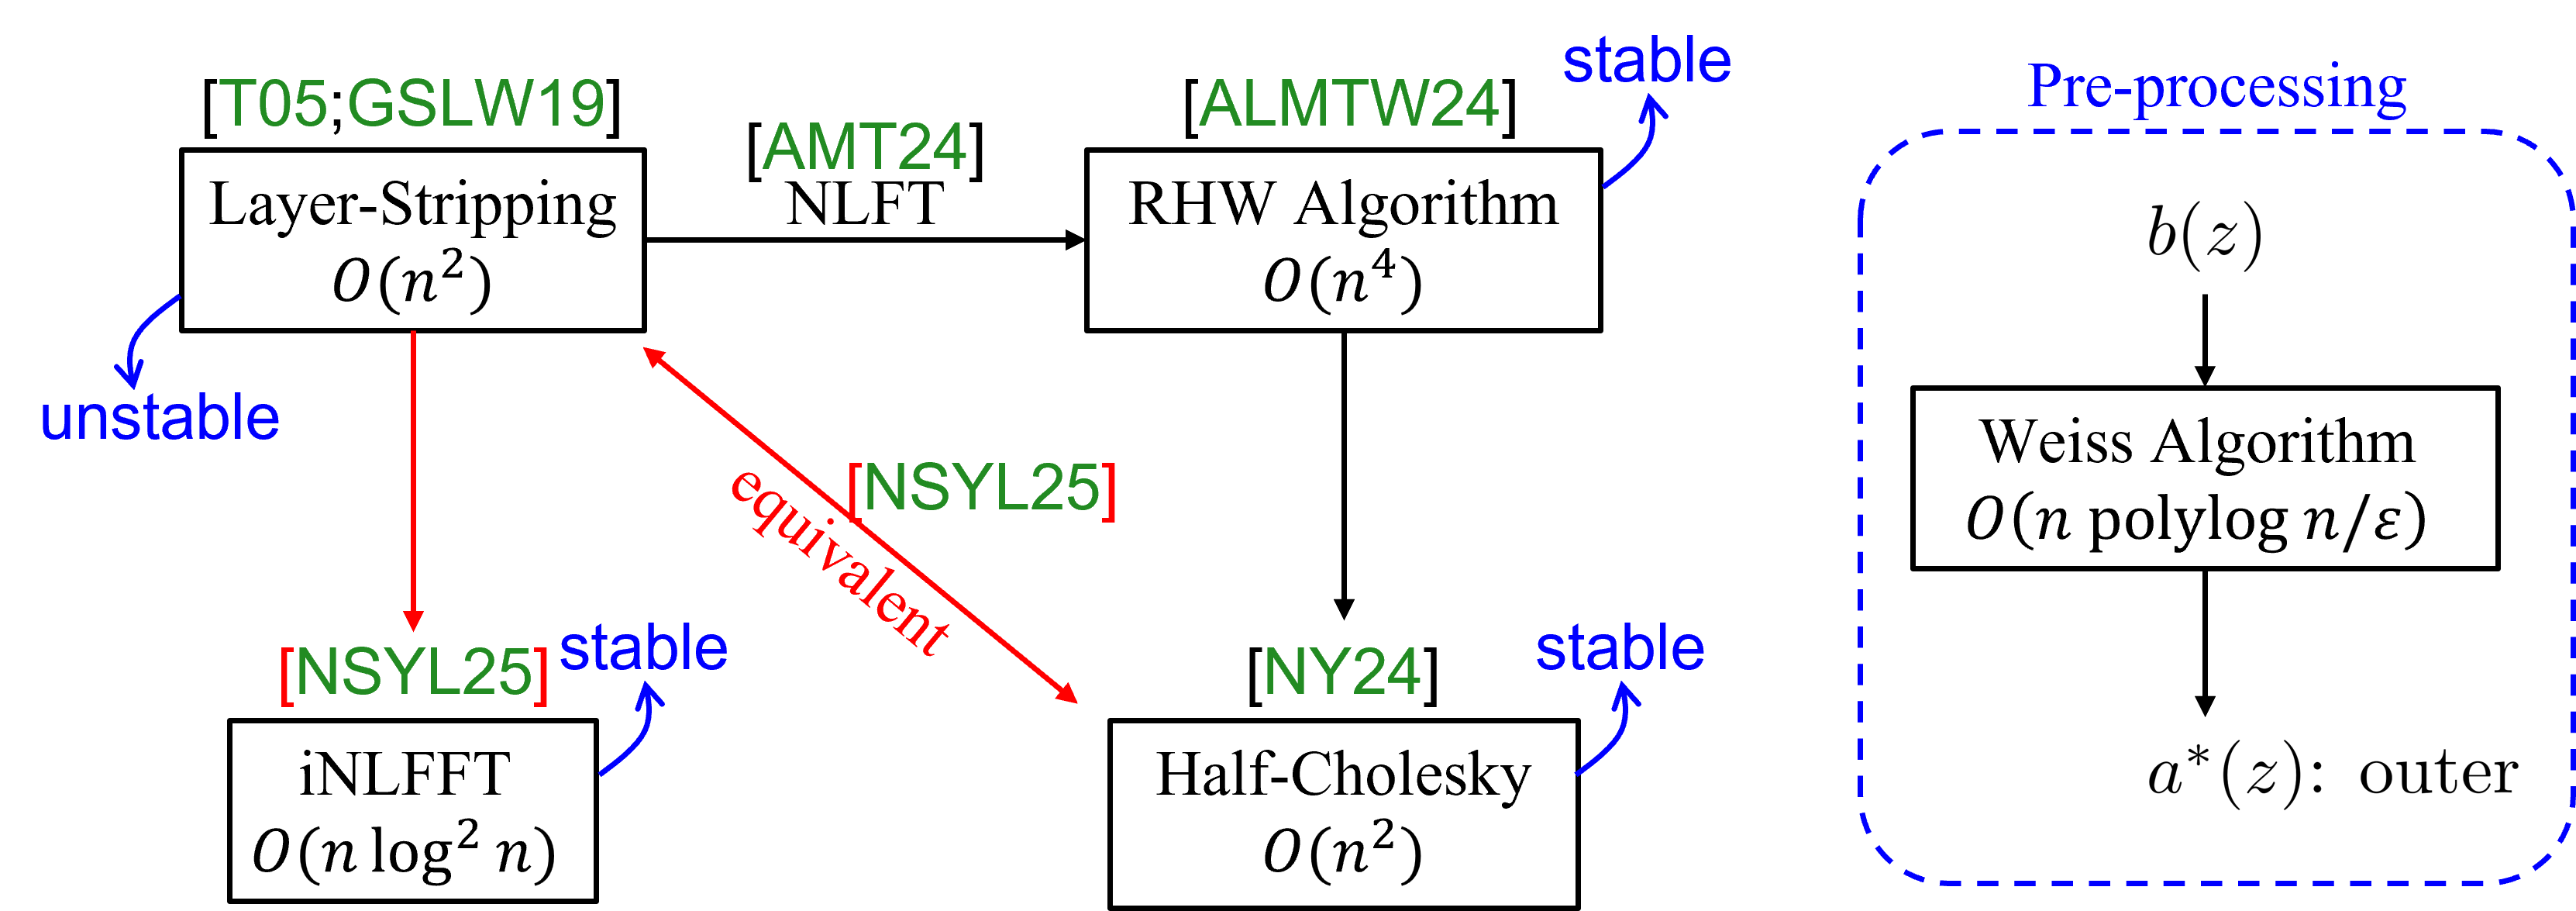
\includegraphics[width=1\linewidth]{figures/roadmap4.png}
    \end{figure}
\end{frame}
\addtocounter{framenumber}{-1}
\begin{frame}{Roadmap}
    \begin{figure}
        \centering
        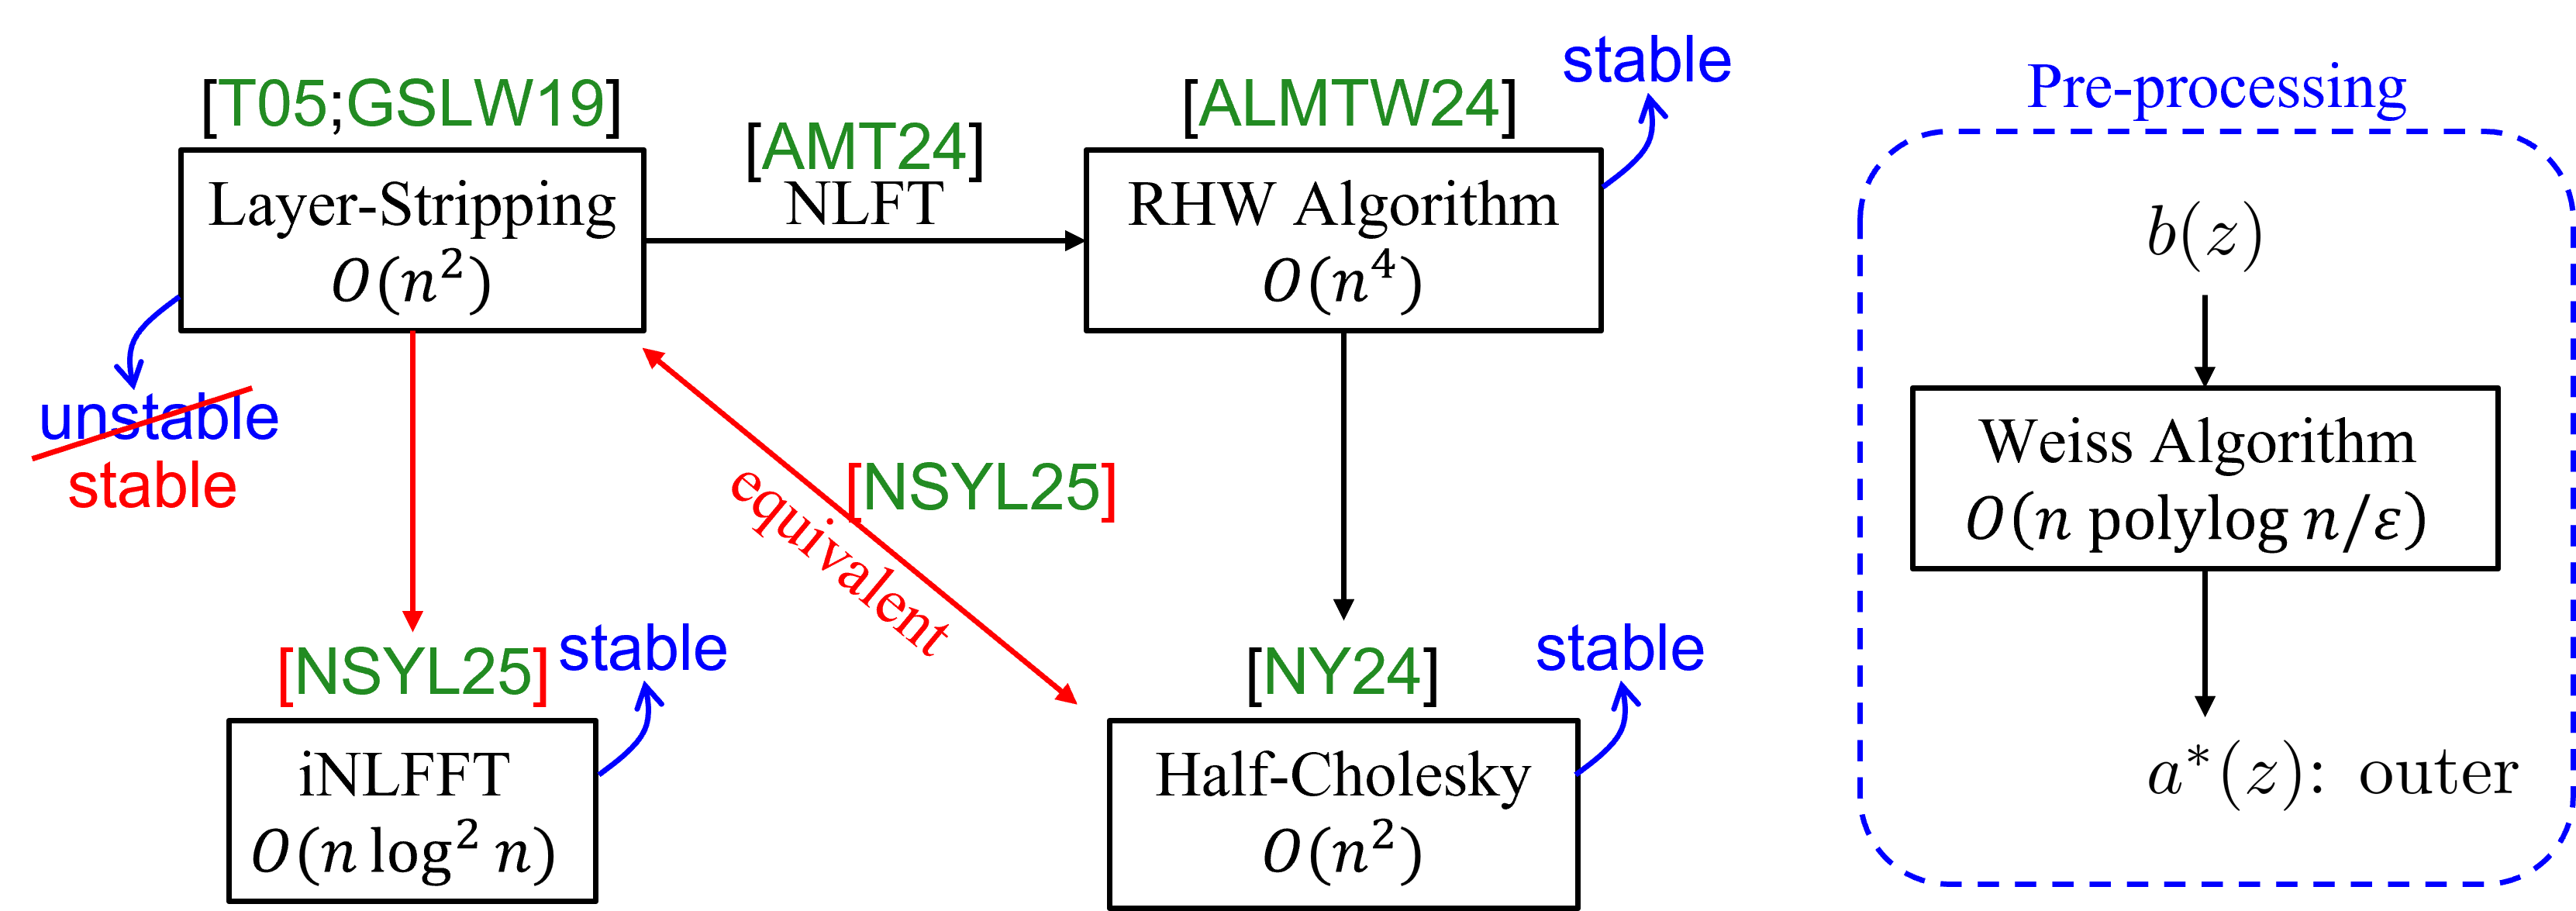
\includegraphics[width=1\linewidth]{figures/roadmap.png}
    \end{figure}
\end{frame}

\subsection{Riemann--Hilbert--Weiss Algorithm}
\begin{frame}{The Scheme}
    This method was proposed in \cite{Szego} under QSP and later generalized to GQSP in \cite{GQSP_NLFT}.
    
    We have seen the layer-stripping method:
    \begin{equation*}
        F_k =  \left.\frac{b_{\ge k}(z) z^{-k}}{a_{\ge k}^*(z)}\right|_{z=0},
    \end{equation*}
    requiring the Riemann--Hilbert factorization
    \begin{equation}
        \left[\begin{matrix}
            1 & P_{\mathbb{D}^*}\frac{b^*}{a^*} \\
            -z^k P_{\mathbbm{D}}z^{-k}\frac{b}{a} & 1
        \end{matrix}\right] \left[\begin{matrix}
            a_{\ge k} \\ b_{\ge k}
        \end{matrix}\right] \propto \left[\begin{matrix}
            1 \\ 0
        \end{matrix}\right].
    \end{equation}
    % \begin{equation}
    %     \underbrace{\left(a(z), b(z)\right)}_{\mathcal{H}^2(\mathbb{D}^*)\times\mathbb{C}[x]} = \underbrace{\left(a_{<k}(z), b_{<k}(z)\right)}_{\mathcal{H}^2(\mathbb{D}^*)\times z^{k-1}\mathcal{H}^2(\mathbb{D}^*)} \underbrace{\left(a_{\ge k}(z), b_{\ge k}(z)\right)}_{\mathcal{H}^2(\mathbb{D}^*)\times \color{red}z^k\mathcal{H}^2(\mathbb{D})}.
    % \end{equation}
    The matrix in the front requires a series representation to $b(z)/a(z)$. This task is accomplished by the \textcolor{blue}{Weiss algorithm}.
\end{frame}

\begin{frame}{Weiss Algorithm}
    Given $b$ that satisfies the \textit{\color{red}Szeg\H{o} condition}, the Weiss algorithm constructs a unique outer $a^*$ such that $(a,b)\in\mathbf{S}$.
    
    Let $R(z) = \log\sqrt{1-\abs{b(z)}^2}$, $G = R + \ii\mathcal{H}(R)$, then $a^* = \exp G$.

    In numerical computation, however, we obtain the Laurent coefficients to $a^*$ by $N=O(n\log (n/\varepsilon))$-point FFT on $R$ and $\exp G$, finally truncating the obtained length-$N$ sequence down to the coefficients representing $z^0$ to $z^n$.

    The complexity of the Weiss algorithm is
    \begin{equation*}
        O(N\log N) = O\left(n\polylog(n/\varepsilon)\right).
    \end{equation*}
\end{frame}

\begin{frame}{Riemann--Hilbert Factorization}
    Given $c(z) \defeq b(z)/a(z) = \sum_{k=-\infty}^nc_kz^k$, we can rewrite the system of linear equations as
    \begin{equation}
        \left[\begin{matrix}
            \mathbbm{1}_{n-k+1} & -T_k^\dagger \\
            T_k & \mathbbm{1}_{n-k+1}
        \end{matrix}\right] \left[\begin{matrix}
            \vec{b}_k \\ \mathrm{rev}(\vec{a}_k^*)
        \end{matrix}\right] \propto \mathrm{rev}(\vec{e}_0),
    \end{equation}
    with vectors $\vec{e}_0=(1,0,\ldots,0)^\transpose$, $\vec{a}_k^* = (a_{k,0}^*,\ldots,a_{k,n-k}^*)^\transpose$, $\vec{b}_k = (b_{k,0},\ldots,b_{k,n-k})^\transpose$, the operator $\mathrm{rev}(\cdot)$ reversing the order of the vector, and the Toeplitz
    \begin{equation}
        T_k = \left[\begin{matrix}
            c_n^* \\
            \vdots & \ddots \\
            c_{k+1}^* & & \ddots \\
            c_k^* & c_{k+1}^* & \cdots & c_n^*
        \end{matrix}\right].
    \end{equation}
\end{frame}
\begin{frame}{Riemann--Hilbert Factorization}
    Each phase term can be computed in parallel, requiring $O(n^3)$ for inverting the matrix! The total complexity will be $O(n^4)$. Costly! However, we can rewrite it: let $T \defeq T_0$,
    \begin{equation*}
        \underbrace{\left[\begin{array}{c:c}
            \mathbbm{1}_{n+1} & -T^\dagger \\ \hdashline
            T & \mathbbm{1}_{n+1}
        \end{array}\right]}_{A} \underbrace{\left[\begin{array}{c:cccc}
            & \color{red}b_{n,0} & \color{red}b_{n-1,0} & \color{red}\cdots & \color{red}b_{0,0} \\
            \mathbbm{1}_{n+1} & & b_{n-1,1} & & \vdots \\
            & & & \ddots & b_{0,n} \\ \hdashline
            & \color{red}a_{n,0}^* & a_{n-1,1}^* & \cdots & a_{0,n}^* \\
            0 & & \color{red}a_{n-1,0}^* & & \vdots \\
            & & & \color{red}\ddots & \color{red}a_{0,0}^*
        \end{array}\right]}_{S} = \underbrace{\left[\begin{array}{c:ccc}
            \mathbbm{1}_{n+1} & & 0 \\ \hdashline
            & * \\
            T & \vdots & \ddots \\
            & * & \cdots & *
        \end{array}\right]}_{L}.
    \end{equation*}
    This is the LU decomposition of $A=LS^{-1}$. The complexity is down to $O(n^3)$.
\end{frame}

%%%%%%%%%%%%%%%%%%%%%%%%%%%%%%%%%%%%%%%%
\subsection{Half-Cholesky Method}
\begin{frame}{Half-Cholesky Method}
    The LU decomposition of $A$ can be written as
    \begin{equation*}
        \left[\begin{matrix}
            \mathbbm{1} & -T^\dagger \\ T & \mathbbm{1}
        \end{matrix}\right] = \left[\begin{matrix}
            \mathbbm{1} \\ T & \mathbbm{1}
        \end{matrix}\right] \left[\begin{matrix}
            \mathbbm{1} \\ & \mathbbm{1}+TT^\dagger
        \end{matrix}\right] \left[\begin{matrix}
            \mathbbm{1} & -T^\dagger \\ & \mathbbm{1}
        \end{matrix}\right].
    \end{equation*}
    If we can obtain the Cholesky decomposition of $\mathbbm{1} + TT^\dagger = LDL^\dagger$, then
    \begin{equation}
        A = \left[\begin{matrix}
            \mathbbm{1} \\ T & L
        \end{matrix}\right] \cdot \left[\begin{matrix}
            \mathbbm{1} \\ & DL^\dagger
        \end{matrix}\right] \left[\begin{matrix}
            \mathbbm{1} & -T^\dagger \\ & \mathbbm{1}
        \end{matrix}\right] \Rightarrow S = \left[\begin{matrix}
            \mathbbm{1} & T^\dagger (DL^\dagger)^{-1} \\
            0 & (DL^\dagger)^{-1}
        \end{matrix}\right].
    \end{equation}
    The general time complexity required for Cholesky decomposition is $O(n^3)$.
\end{frame}
\begin{frame}{Half-Cholesky Method}
    We don't need to do the whole Cholesky decomposition, however, as what we need is
    \begin{align}
        \left[\begin{matrix}
            a_{n,0} \\ \vdots \\ a_{0,0}
        \end{matrix}\right] &\propto D^{-1} \left[\begin{matrix}
            1 \\ \vdots \\ 1
        \end{matrix}\right] \text{ and }
        \left[\begin{matrix}
            b_{n,0} \\ \vdots \\ b_{0,0}
        \end{matrix}\right] \propto D^{-1}L^{-*} \vec{c}_0 \text{, with } \vec{c}_0 = \left[\begin{matrix}
            c_n \\ \vdots \\ c_0
        \end{matrix}\right],
    \end{align}
    as $\mathbbm{1}+TT^\dagger\succeq 0$, $D$ is real. The proportionality constant for the two equations above are the same. The Fourier coefficients will be
    \begin{equation}
        \left[\begin{matrix}
            F_n \\ \vdots \\ F_0
        \end{matrix}\right] = \left[\begin{matrix}
            b_{n,0}/a_{n,0} \\ \vdots \\ b_{0,0}/a_{0,0}
        \end{matrix}\right] = L^{-*} \vec{c}_0.
    \end{equation}
    
\end{frame}
\begin{frame}{Half-Cholesky Method}
    \begin{columns}
    \begin{column}{0.5\textwidth}
        For the Cholesky decomposition of $\mathbbm{1}+TT^\dagger$, we can do better than $O(n^3)$! Observe that $T$ is a Toeplitz, it can be fully characterized by $n\times 2$ numbers. Hence, we can expect that the LDL decomposition of $\mathbbm{1}+TT^\dagger$ should be faster!
        \begin{remark}[Displacement]
            If the \textit{displacement rank} of an $n\times n$ matrix is $r$, then the Cholesky decomposition has complexity $O(n^2r)$.
        \end{remark}
        Hence, the final complexity for the half-Cholesky method is $O(n^2)$
    \end{column}
    \begin{column}{0.5\textwidth}
        \begin{equation}
            Z \defeq \left[\begin{matrix}
                0 \\
                1 & 0 \\
                & \ddots & \ddots \\
                & & 1 & 0
            \end{matrix}\right]
        \end{equation}
        For $K=\mathbbm{1} + TT^\dagger$,
        \begin{align}
            \Delta K &\defeq K - ZKZ^\transpose = \vec{e}_0\vec{e}_0^\dagger + \vec{c}_0\vec{c}_0^\dagger \\
            &= \left[\begin{matrix}
                \vec{e}_0 & \vec{c}_0
            \end{matrix}\right] \left[\begin{matrix}
                \vec{e}_0^\dagger \\ \vec{c}_0^\dagger
            \end{matrix}\right] = G_0G_0^\dagger.
        \end{align}
        The displacement rank $r=2$ \cite{SAYED199549}.
    \end{column}
    \end{columns}
\end{frame} 


\subsection{Layer-Stripping Revisited}
\begin{frame}{Layer-Stripping Revisited}
    Let us follow \cite{Lin2025} and rewrite layer-stripping in a matrix notation:
    \begin{align*}
        \left(a_{\ge k},b_{\ge k}\right) &= \frac{1}{\sqrt{1+\abs{F_k}^2}} \left(1,F_kz^k\right) \left(a_{\ge k+1},b_{\ge k+1}\right) \\
        \Rightarrow \left(a_{\ge k+1},b_{\ge k+1}\right) &= \frac{1}{\sqrt{1+\abs{F_k}^2}} \left(1,-F_kz^k\right) \left(a_{\ge k},b_{\ge k}\right)
    \end{align*}
    Thus, we have
    \begin{align}
        {\color{teal} a_{\ge k+1}^*} &= \frac{1}{\sqrt{1+\abs{F_k}^2}} \left({\color{teal} a_{\ge k}^*} + \overline{F}_k {\color{blue} z^{-k}b_{\ge k}}\right), \\
        {\color{blue} z^{-(k+1)}b_{\ge k+1}} &= \frac{1}{{\color{red}z}\sqrt{1+\abs{F_k}^2}} \left(-F_k {\color{teal} a_{\ge k}^*} + {\color{blue} z^{-k}b_{\ge k}}\right).
    \end{align}
\end{frame}
\begin{frame}{Layer-Stripping Revisited}
    Through the parameterization ${\color{teal}a_{\ge k}^*} = \sum_{j=0}^{n-k} {\color{teal}a_{k,j}} z^j$ and ${\color{blue}z^{-k}b_{\ge k}} = \sum_{j=0}^{n-k} {\color{blue}b_{k,j}} z^j$, we have
    \begin{equation}
        \left[\begin{matrix}
            \color{teal}a_{k+1,0} & \color{black}0 \\
            \color{teal}a_{k+1,1} & \color{blue}b_{k+1,0} \\
            \color{teal}\vdots & \color{blue}\vdots \\
            \color{teal}a_{k+1,n-k-1} & \color{blue}b_{k+1,n-k-2} \\
            {\color{red}0} & \color{blue}b_{k+1,n-k-1}
        \end{matrix}\right] = \underbrace{\left[\begin{matrix}
            \color{teal}a_{k,0} & \color{blue}b_{k,0} \\
            \color{teal}a_{k,1} & \color{blue}b_{k,1} \\
            \color{teal}\vdots & \color{blue}\vdots \\
            \color{teal}a_{k,n-k-1} & \color{blue}b_{k,n-k-1} \\
            \color{teal}a_{k,n-k} & \color{blue}b_{k,n-k}
        \end{matrix}\right]}_{G_{k} = [{\color{teal}\vec{a}_k},{\color{blue}\vec{b}_k}]} \frac{1}{\sqrt{1+\abs{F_k}^2}} \left[\begin{matrix}
            1 & -F_k \\ \overline{F}_k & 1
        \end{matrix}\right]
    \end{equation}
    The phase $F_k = {\color{blue}b_{k,0}}/{\color{teal}a_{k,0}}$ is obtained by the QR decomposition of $G_k$, requiring $O(n)$ complexity each. The total complexity will be $O(n^2)$.
\end{frame}
\begin{frame}{Layer-Stripping Revisited}
    However, through induction, we see that for any $f(z)$, the following sequence has the same layer-stripped Fourier coefficients:
    \begin{equation*}
        \left(a(z)/f(z) , b(z)/f(z)\right).
    \end{equation*}

    The layer-stripping method is closely related to the half-Cholesky method previously mentioned when setting $f = a$, then the half-Cholesky method is just applying layer-stripping on
    \begin{equation*}
        \left(1,b(z)/a(z)\right) \eqdef \left(1,c(z)\right).
    \end{equation*}
\end{frame}

\subsection{Inverse Nonlinear FFT}
\begin{frame}{Inverse Nonlinear FFT}
    This is the state-of-the-art proposed by \cite{Lin2025} on May 19th, 2025. It essentially reduces the redundancy in computation of the layer-stripping method (or equivalently, the half-Cholesky method).

    Though inspired by \cite{FastToeplitz}, it's essence is still, nevertheless, layer-stripping:
    \begin{equation}
        \left[\begin{matrix}
            \color{teal}a_{k+1,0} & \color{black}0 \\
            \color{teal}a_{k+1,1} & \color{blue}b_{k+1,0} \\
            \color{teal}\vdots & \color{blue}\vdots \\
            \color{teal}a_{k+1,n-k-1} & \color{blue}b_{k+1,n-k-2} \\
            {\color{red}0} & \color{blue}b_{k+1,n-k-1}
        \end{matrix}\right] = \underbrace{\left[\begin{matrix}
            \color{teal}a_{k,0} & \color{blue}b_{k,0} \\
            \color{teal}a_{k,1} & \color{blue}b_{k,1} \\
            \color{teal}\vdots & \color{blue}\vdots \\
            \color{teal}a_{k,n-k-1} & \color{blue}b_{k,n-k-1} \\
            \color{teal}a_{k,n-k} & \color{blue}b_{k,n-k}
        \end{matrix}\right]}_{G_{k} = [{\color{teal}\vec{a}_k},{\color{blue}\vec{b}_k}]} \frac{1}{\sqrt{1+\abs{F_k}^2}} \left[\begin{matrix}
            1 & -F_k \\ \overline{F}_k & 1
        \end{matrix}\right].
    \end{equation}
\end{frame}
\begin{frame}{Inverse Nonlinear FFT}
    The previous algorithm (layer-stripping, or equivalently, half-Cholesky) follows:
    \begin{equation*}
        G_0=[\vec{a}_0,\vec{b}_0] \longmapsto G_1=[\vec{a}_1,\vec{b}_1] \longmapsto \cdots \longmapsto G_{\ceil{n/2}} \longmapsto \cdots \longmapsto G_n,
    \end{equation*}
    where each arrow represents a QR decomposition and shifting.

    Note that the calculation to $(F_{\ceil{n/2}},\ldots,F_n)$ fully depends on $G_{\ceil{n/2}}$, with $G_{\ceil{n/2}}$ depending on $(F_0,\ldots,F_{\ceil{n/2}-1})$.

    Similarly, we can continue this partitioning process.
    
\end{frame}

\begin{frame}{Inverse Nonlinear FFT}
    \vspace{0.3cm}
    \begin{figure}
        \centering
        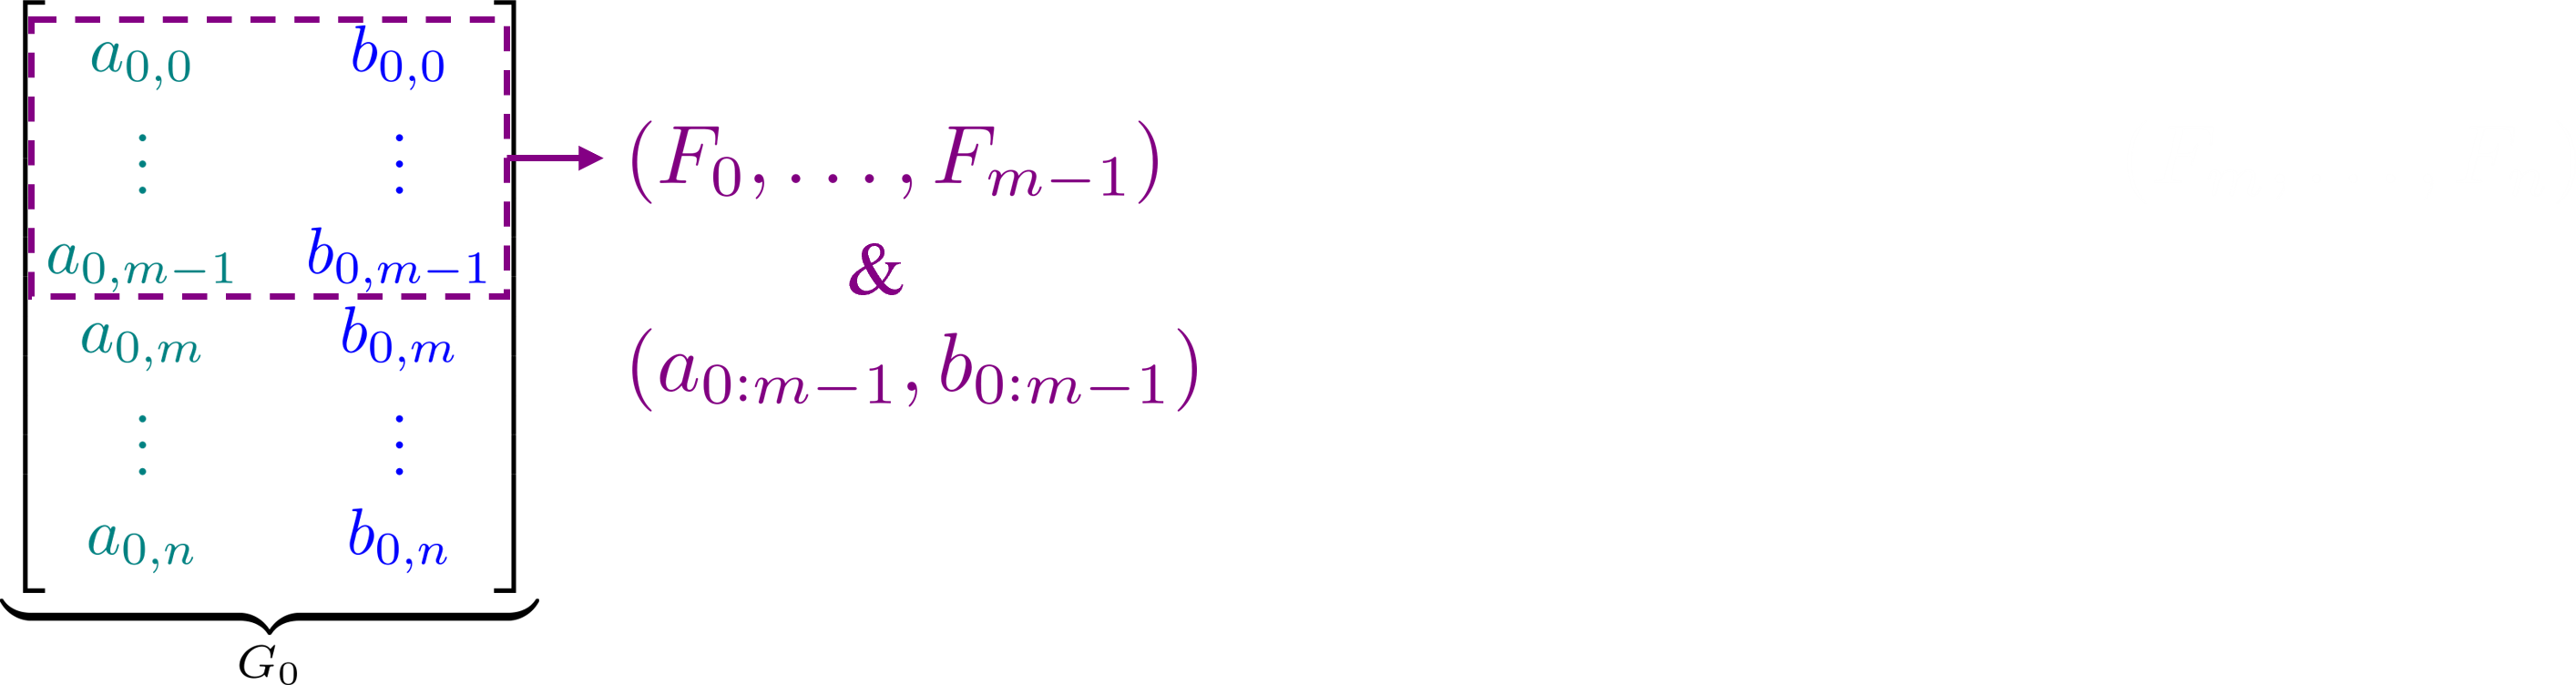
\includegraphics[height=0.24\textwidth]{figures/iNLFFT2.png}
        % \caption{Caption}
        % \label{fig:enter-label}
    \end{figure}
    
    \color{white}The time complexity required for calculating
    \begin{equation*}
        G_m = (a_{m:n},b_{m:n}) = (a_{0:m-1},b_{0:m-1})^{-1} (a_{0:n},b_{0:n}) = (a_{0:m-1},b_{0:m-1})^{-1} G_0,
    \end{equation*}
    where $m=\ceil{n/2}$, is $O(n\log n)$. The total time complexity is
    \begin{equation}
        n\log n + 2\left(\frac{n}{2}\log\frac{n}{2}\right) + 4\left(\frac{n}{4}\log\frac{n}{4}\right) + \cdots = O(n\log^2n).
    \end{equation}
\end{frame}
\addtocounter{framenumber}{-1}
\begin{frame}{Inverse Nonlinear FFT}
    \vspace{0.3cm}
    \begin{figure}
        \centering
        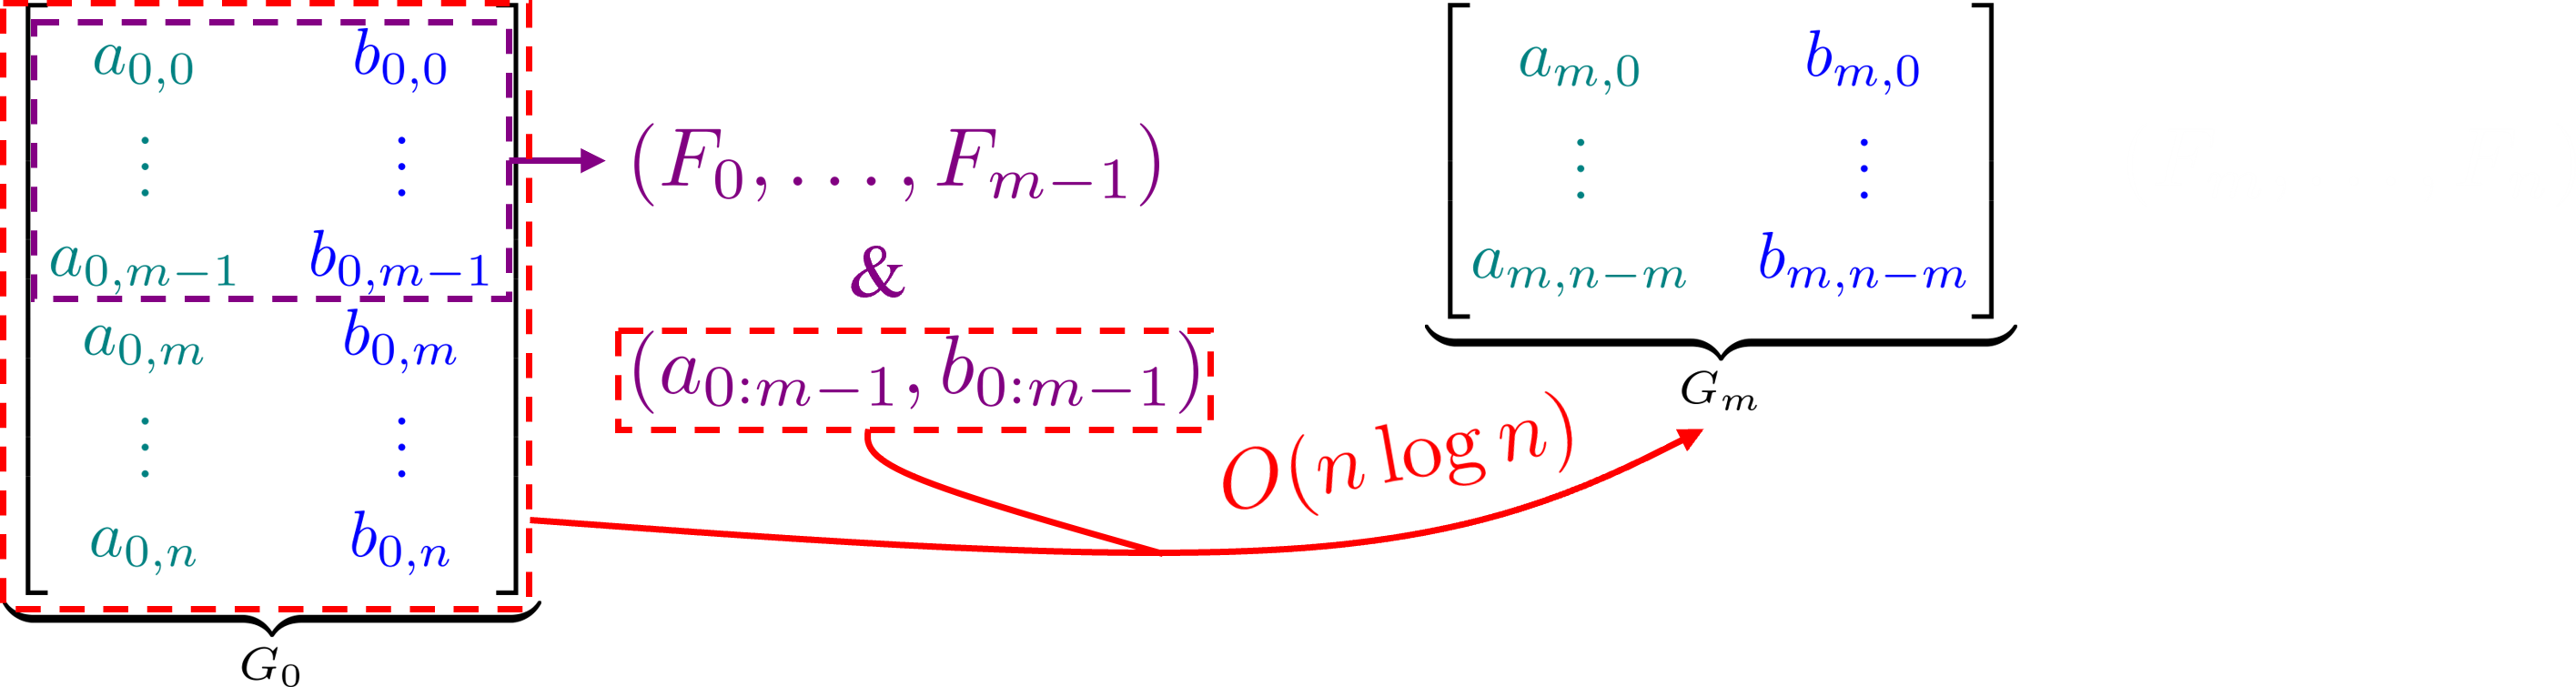
\includegraphics[height=0.24\textwidth]{figures/iNLFFT3.png}
        % \caption{Caption}
        % \label{fig:enter-label}
    \end{figure}
    
    The time complexity required for calculating
    \begin{equation*}
        G_m = (a_{m:n},b_{m:n}) = (a_{0:m-1},b_{0:m-1})^{-1} (a_{0:n},b_{0:n}) = (a_{0:m-1},b_{0:m-1})^{-1} G_0,
    \end{equation*}
    where $m=\ceil{n/2}$, is $O(n\log n)$. \color{white}The total time complexity is
    \begin{equation}
        n\log n + 2\left(\frac{n}{2}\log\frac{n}{2}\right) + 4\left(\frac{n}{4}\log\frac{n}{4}\right) + \cdots = O(n\log^2n).
    \end{equation}
\end{frame}
\addtocounter{framenumber}{-1}
\begin{frame}{Inverse Nonlinear FFT}
    \vspace{0.3cm}
    \begin{figure}
        \centering
        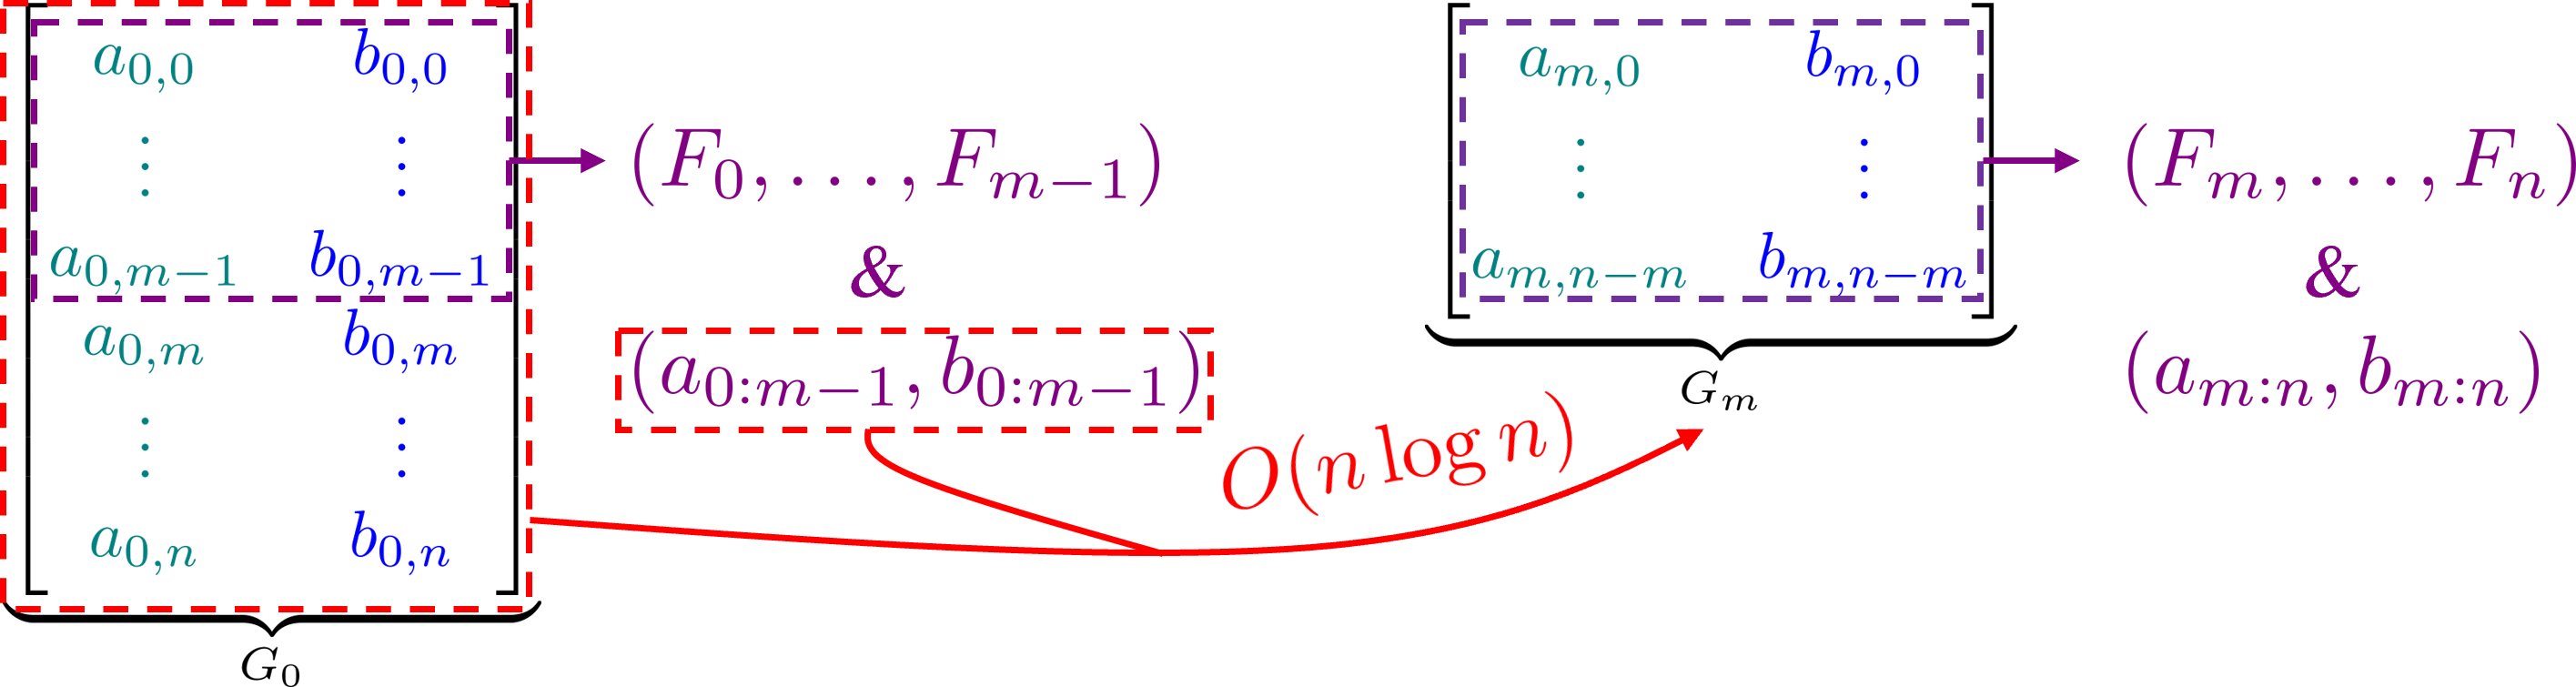
\includegraphics[height=0.24\textwidth]{figures/iNLFFT.png}
        % \caption{Caption}
        % \label{fig:enter-label}
    \end{figure}
    
    The time complexity required for calculating
    \begin{equation*}
        G_m = (a_{m:n},b_{m:n}) = (a_{0:m-1},b_{0:m-1})^{-1} (a_{0:n},b_{0:n}) = (a_{0:m-1},b_{0:m-1})^{-1} G_0,
    \end{equation*}
    where $m=\ceil{n/2}$, is $O(n\log n)$. The total time complexity is
    \begin{equation}
        n\log n + 2\left(\frac{n}{2}\log\frac{n}{2}\right) + 4\left(\frac{n}{4}\log\frac{n}{4}\right) + \cdots = O(n\log^2n).
    \end{equation}
\end{frame}